\documentclass[../../compsys.tex]{subfiles}
\begin{document}

\chapter{Client/Server Model \& The Web}
\textit{Network ! Back to our Youtube example. (sorry for the delay was working on something else, I hope midterm went not too bad.)}\\
\vfill
\section*{Introduction}
This chapter introduces the client/server model, a foundational concept of the modern web. We use YouTube as an example: when you play a video, your browser (client) communicates with a YouTube server to stream content. These two separate processes exchange messages over the network, forming a distributed application.

\begin{center}
    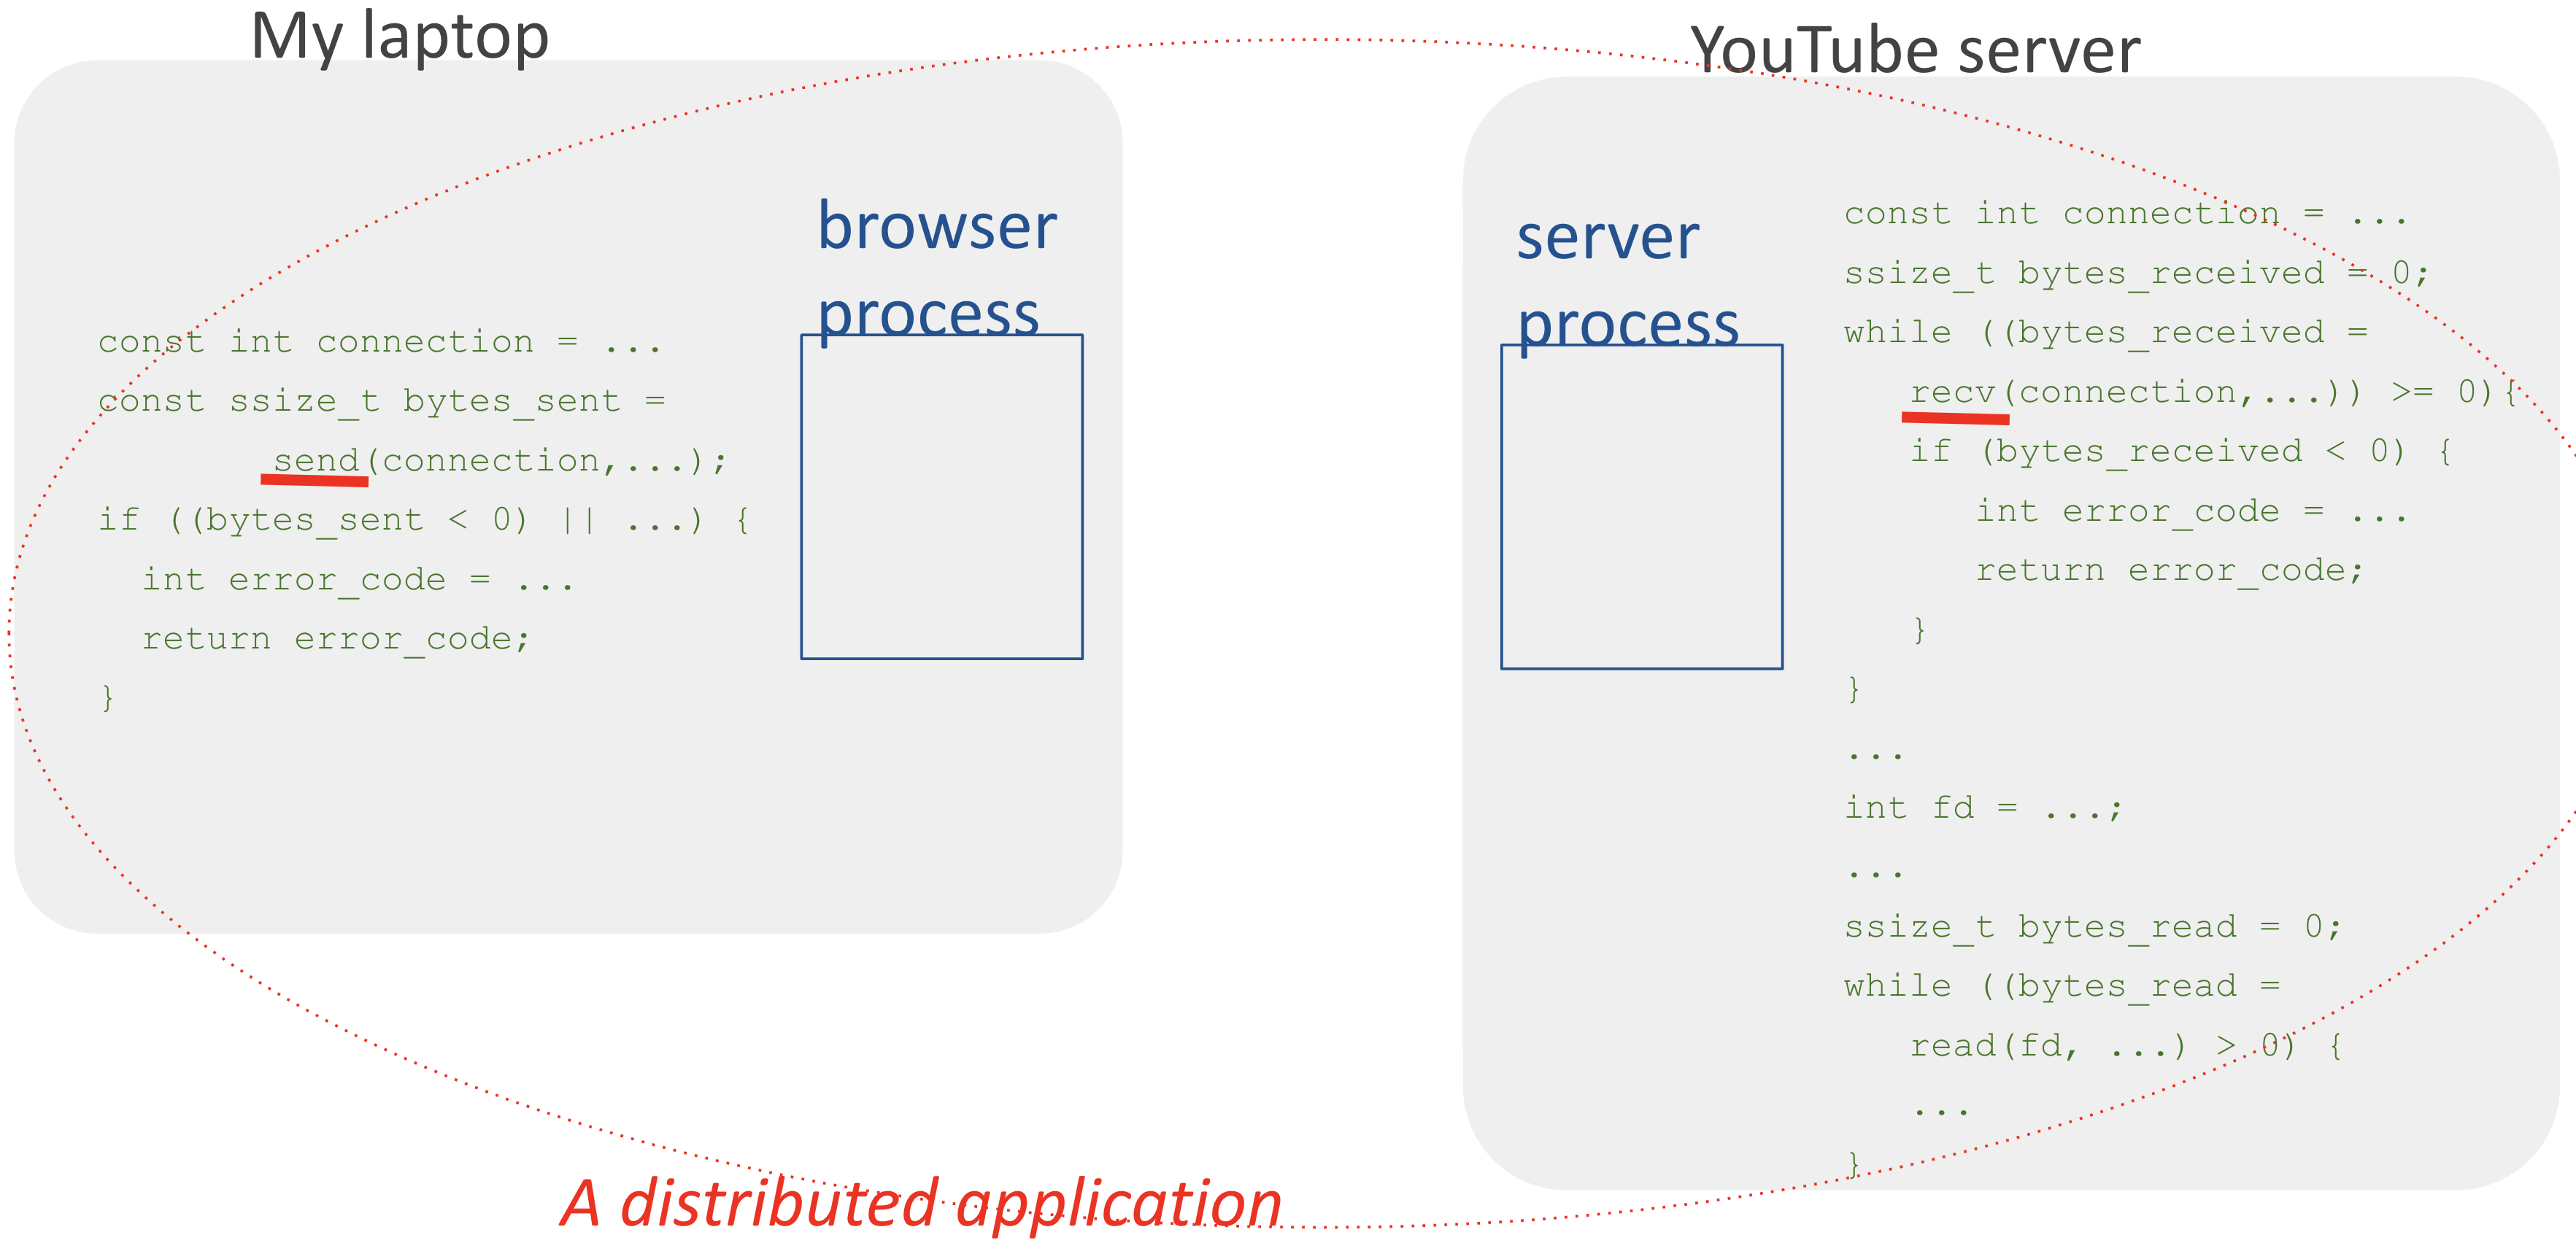
\includegraphics[width=0.8\textwidth]{images/youtube.png}
\end{center}

\section{Distributed Applications}
A \textbf{distributed application} consists of:
\begin{itemize}
    \item[-] Processes running on different computers,
    \item[-] Exchanging messages over a network,
    \item[-] Collaborating to achieve a shared goal.
\end{itemize}
\newpage
\section{Client/Server Architecture}
Most distributed applications use a client/server architecture:
\begin{itemize}
    \item One process acts as the \textbf{client}, making requests.
    \item Another acts as the \textbf{server}, responding to requests.
\end{itemize}
\begin{center}
    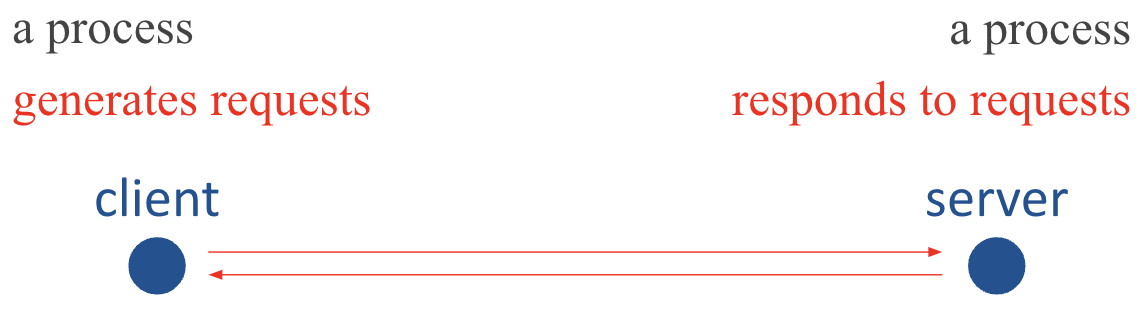
\includegraphics[width=0.7\textwidth]{images/client-server.png}
\end{center}
Clients and servers have clearly defined roles. Servers typically run on dedicated infrastructure, which today often means multiple data centers and many server processes.

\subsection{Naming and Identifying Processes}
To communicate, client and server processes need unique identifiers:
\begin{itemize}
    \item[-] \textbf{Local identifiers} (e.g., process ID or PID) only have meaning within a single computer.
    \item[-] \textbf{Global identifiers} are needed for communication across computers.
\end{itemize}

\begin{center}
    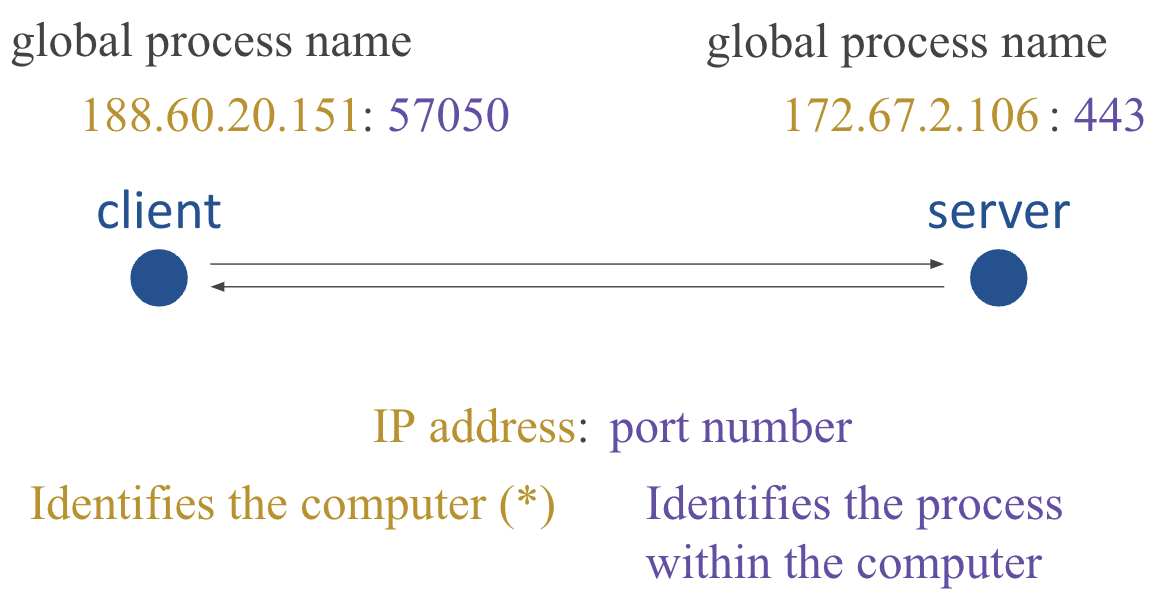
\includegraphics[width=0.6\textwidth]{images/process-view.png}
\end{center}

A global process name consists of:
\begin{itemize}
    \item[-] An \textbf{IP address} — uniquely identifies a computer (e.g., \texttt{172.67.2.106}),
    \item[-] A \textbf{port number} — uniquely identifies a process on that computer (e.g., \texttt{443}, \texttt{57057}).
\end{itemize}

An IP address is like a street name; a port number is like a house number. Together, they uniquely identify a process on the network.
\newpage
\subsection{Discovering the Server Process}

Before communication can begin, the client must discover the server's global name (IP address and port number). Once known, the client can initiate contact by introducing itself to the server.

\vspace{0.5em}
\begin{center}
    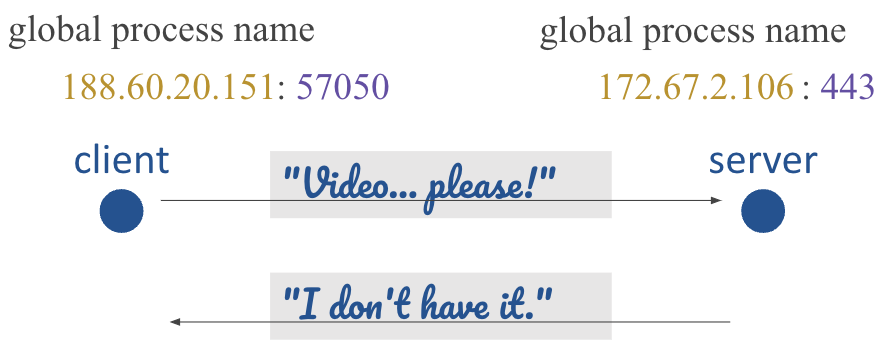
\includegraphics[width=0.6\textwidth]{images/notfound.png}
\end{center}
Suppose the client requests a video from the server, but the server does not have the requested video. The server replies with a message indicating the resource is not found (for example, an HTTP 404 error).

\vspace{0.5em}
\begin{center}
    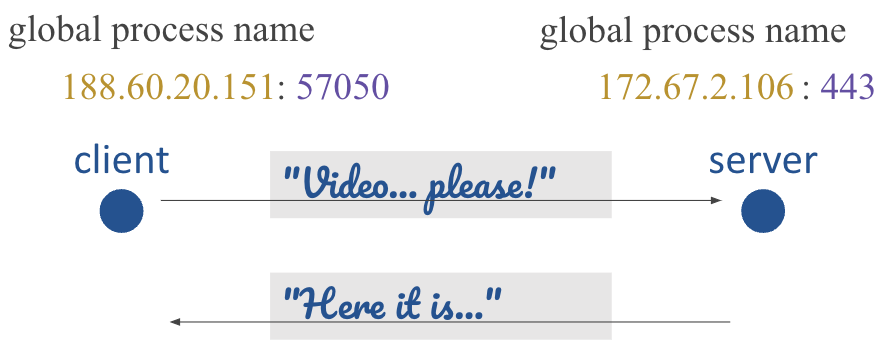
\includegraphics[width=0.6\textwidth]{images/success.png}
\end{center}
If the server has the video, it responds with the requested data (such as an HTTP 200 OK response), and the client can begin receiving the video stream.

\vspace{0.5em}
\begin{center}
    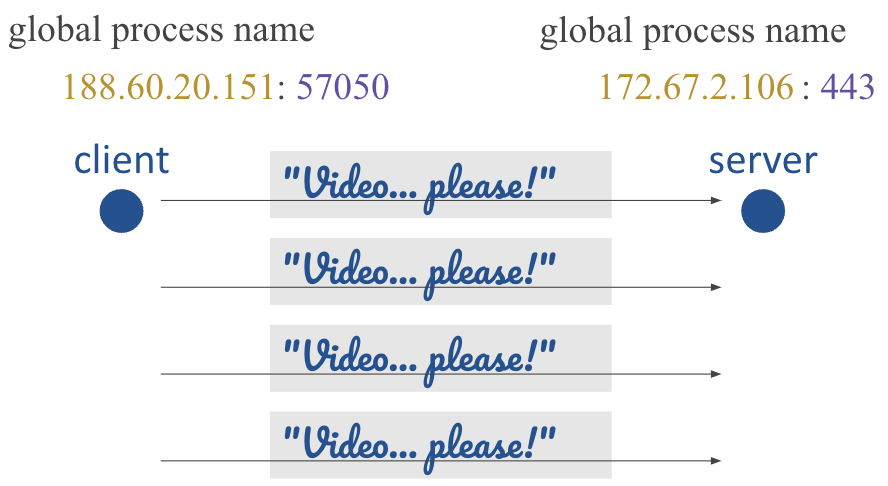
\includegraphics[width=0.6\textwidth]{images/violating.png}
\end{center}
If the client does not follow the expected protocol—such as repeatedly sending requests for the same video without waiting for a response—the server may choose to ignore these requests or terminate the connection. This is a \textbf{protocol violation}.\\
Once the client knows the server's address, they can exchange messages according to a \textbf{communication protocol}.

\subsection{Communication Protocols}

A \textbf{communication protocol} defines the set of valid interactions between client and server processes. For example, a typical protocol might allow:

\begin{itemize}
    \item The client requests information; the server responds with the requested data.
    \item The client requests information; the server responds that the information is unavailable.
\end{itemize}

If either party sends an unexpected or invalid message—such as the client repeating the same request rapidly—the protocol is violated. In such cases, the server may choose not to respond or may close the connection.

\medskip

\noindent
\textit{Analogy:} Communication protocols in computers are similar to social protocols in conversation. If someone repeatedly asks questions without waiting for answers, the other person may stop responding.

\medskip

\noindent
\textbf{Summary:} Communication between distributed processes is only possible when the client can discover the server's address and both sides follow an agreed protocol. Violating the protocol typically ends the communication.
\section{The HyperText Transfer Protocol (HTTP)}
The HyperText Transfer Protocol (HTTP) is the foundation of communication on the World Wide Web. It defines how web clients (e.g., browsers) and web servers exchange information.

\subsection{HTTP Requests and Responses}
\begin{itemize}[label=$\bullet$]
    \item \textbf{Request}: A web client sends an HTTP request to a server to retrieve or manipulate resources.
    \item \textbf{Response}: The web server processes the request and returns an HTTP response.
    \item \textbf{Common Request Methods}:
        \begin{itemize}[label=--]
            \item \texttt{GET}: Retrieves a specified resource.
            \item \texttt{HEAD}: Retrieves metadata about a resource without the resource itself (e.g., object size or type).
            \item \texttt{POST}: Sends data to the server, often used for form submissions.
        \end{itemize}
    \item \textbf{Common Response Status Codes}:
        \begin{itemize}[label=--]
            \item \texttt{200 OK}: Request was successful.
            \item \texttt{404 Not Found}: Requested resource could not be found.
            \item \texttt{400 Bad Request}: Request was malformed.
            \item \texttt{301 Moved Permanently}: Resource has been relocated to a new URL.
        \end{itemize}
\end{itemize}

\subsection{Web Objects}
A web object is any resource accessible on the web, identified by a unique Uniform Resource Locator (URL).

\begin{itemize}[label=$\bullet$]
    \item[-] \textbf{Types}: Text files, images, videos, scripts, etc.
    \item[-] \textbf{URL Example}: \url{https://actu.epfl.ch/image/142932/1920x1080.jpg}
    \item[-] \textbf{Access}: Retrieved by a web client from a server using an HTTP request (e.g., \texttt{GET /image/142932/1920x1080.jpg}).
    \item[-] \textbf{Uniqueness}: Each URL serves as a globally unique identifier for the resource.
\end{itemize}

\subsection{Web Pages}
A web page is a specific type of web object, typically composed of multiple resources.

\begin{itemize}[label=$\bullet$]
    \item \textbf{Structure}: Consists of a base file (e.g., HTML) that defines the page's structure and references other objects.
    \item \textbf{Referenced Objects}: May include images, videos, scripts, or other web pages.
    \item \textbf{Example}: A web page might include an HTML file, CSS stylesheets, and embedded images, all fetched via separate HTTP requests.
\end{itemize}

\subsection{Designing a Distributed Application}

When developing a distributed application, it is essential to:
\begin{itemize}
    \item Decide how many processes (and threads) are needed, and define the role of each.
    \item Design the communication protocol between the participating processes and threads.
\end{itemize}
These decisions should be made before any coding begins.

\vspace{1em}

A common and universal example of a client/server application is the web:
\begin{itemize}
    \item \textbf{Web clients} (web browsers) generate requests for web resources.
    \item \textbf{Web servers} respond to these requests.
\end{itemize}


The communication protocol between a web client and a web server is the HyperText Transfer Protocol (\textbf{HTTP}), which is based on simple request and response interactions.

\vspace{1em}

The most frequent request type is a \texttt{GET} request. The server can reply in several ways, each shown below:

\begin{center}
    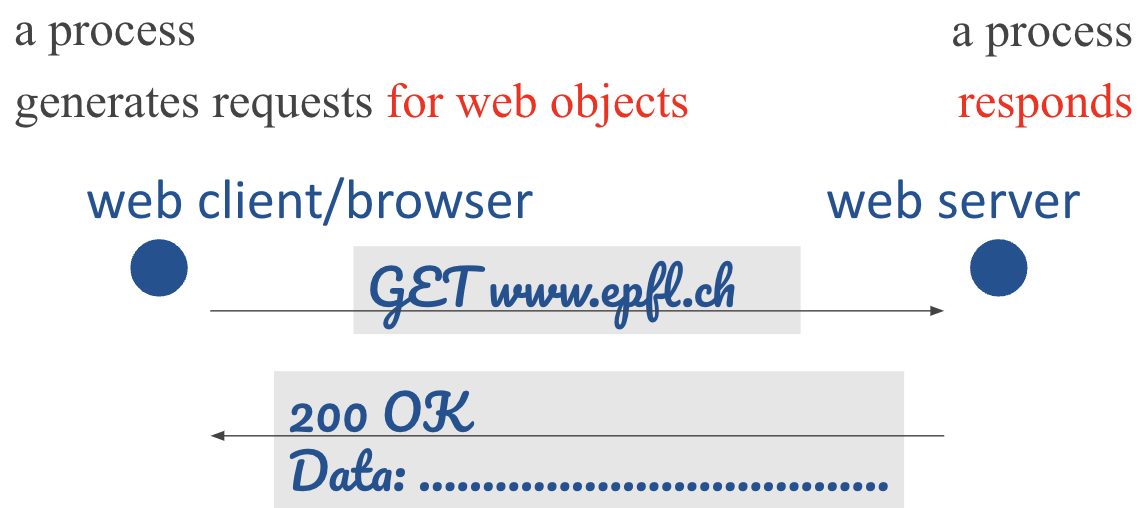
\includegraphics[width=0.6\textwidth]{images/200.png}
\end{center}
When the server has the requested resource, it replies with a \texttt{200 OK} response, providing the object to the client.

\begin{center}
    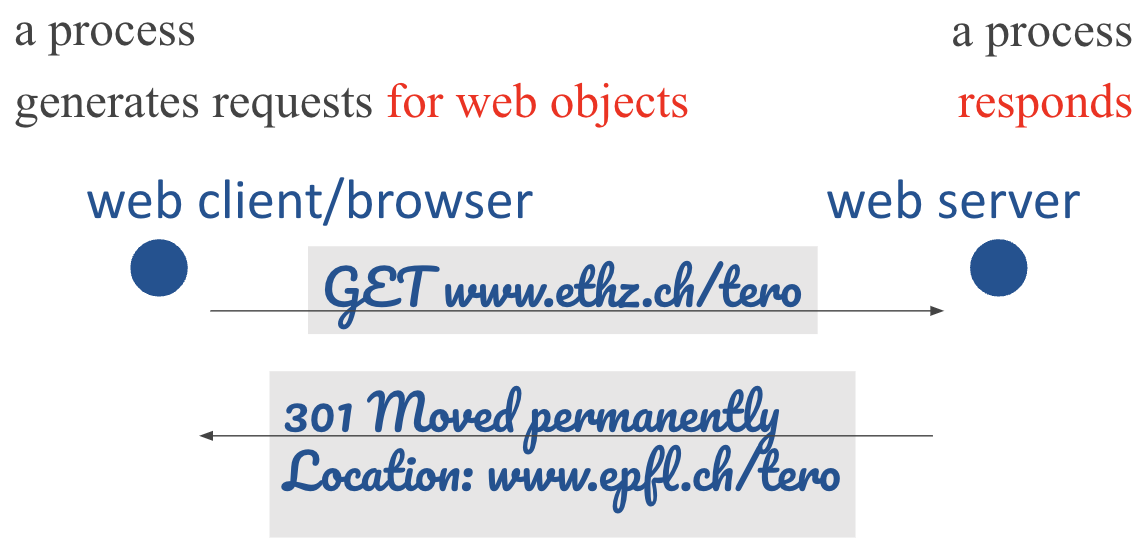
\includegraphics[width=0.6\textwidth]{images/301.png}
\end{center}
If the resource has been moved, the server replies with a \texttt{301 Moved Permanently} response, including the new location.

\begin{center}
    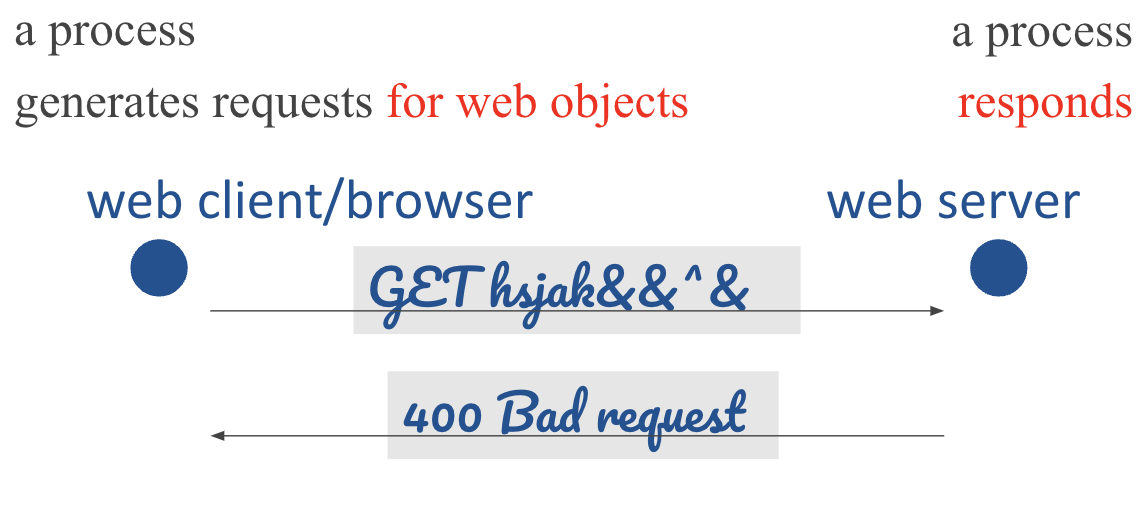
\includegraphics[width=0.6\textwidth]{images/400.png}
\end{center}
If the client's request is malformed or invalid, the server responds with a \texttt{400 Bad Request} error. This is rare in practice, because web browsers typically generate well-formed requests on behalf of users.

\begin{center}
    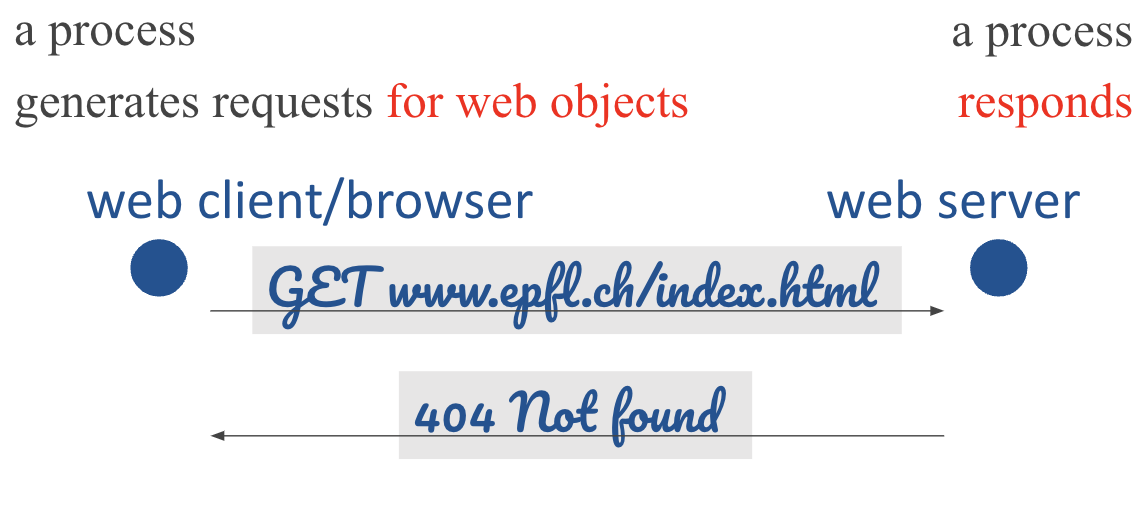
\includegraphics[width=0.6\textwidth]{images/404.png}
\end{center}
If the requested resource does not exist, the server sends a \texttt{404 Not Found} error.

\vspace{1em}

\noindent
\textit{Note:} Most protocol errors are handled by the browser itself and are not directly seen by the user.
\subsection{Example: Common Web Client/Server Exchanges}
\begin{minipage}[htp]{0.45\textwidth}
\begin{center}
    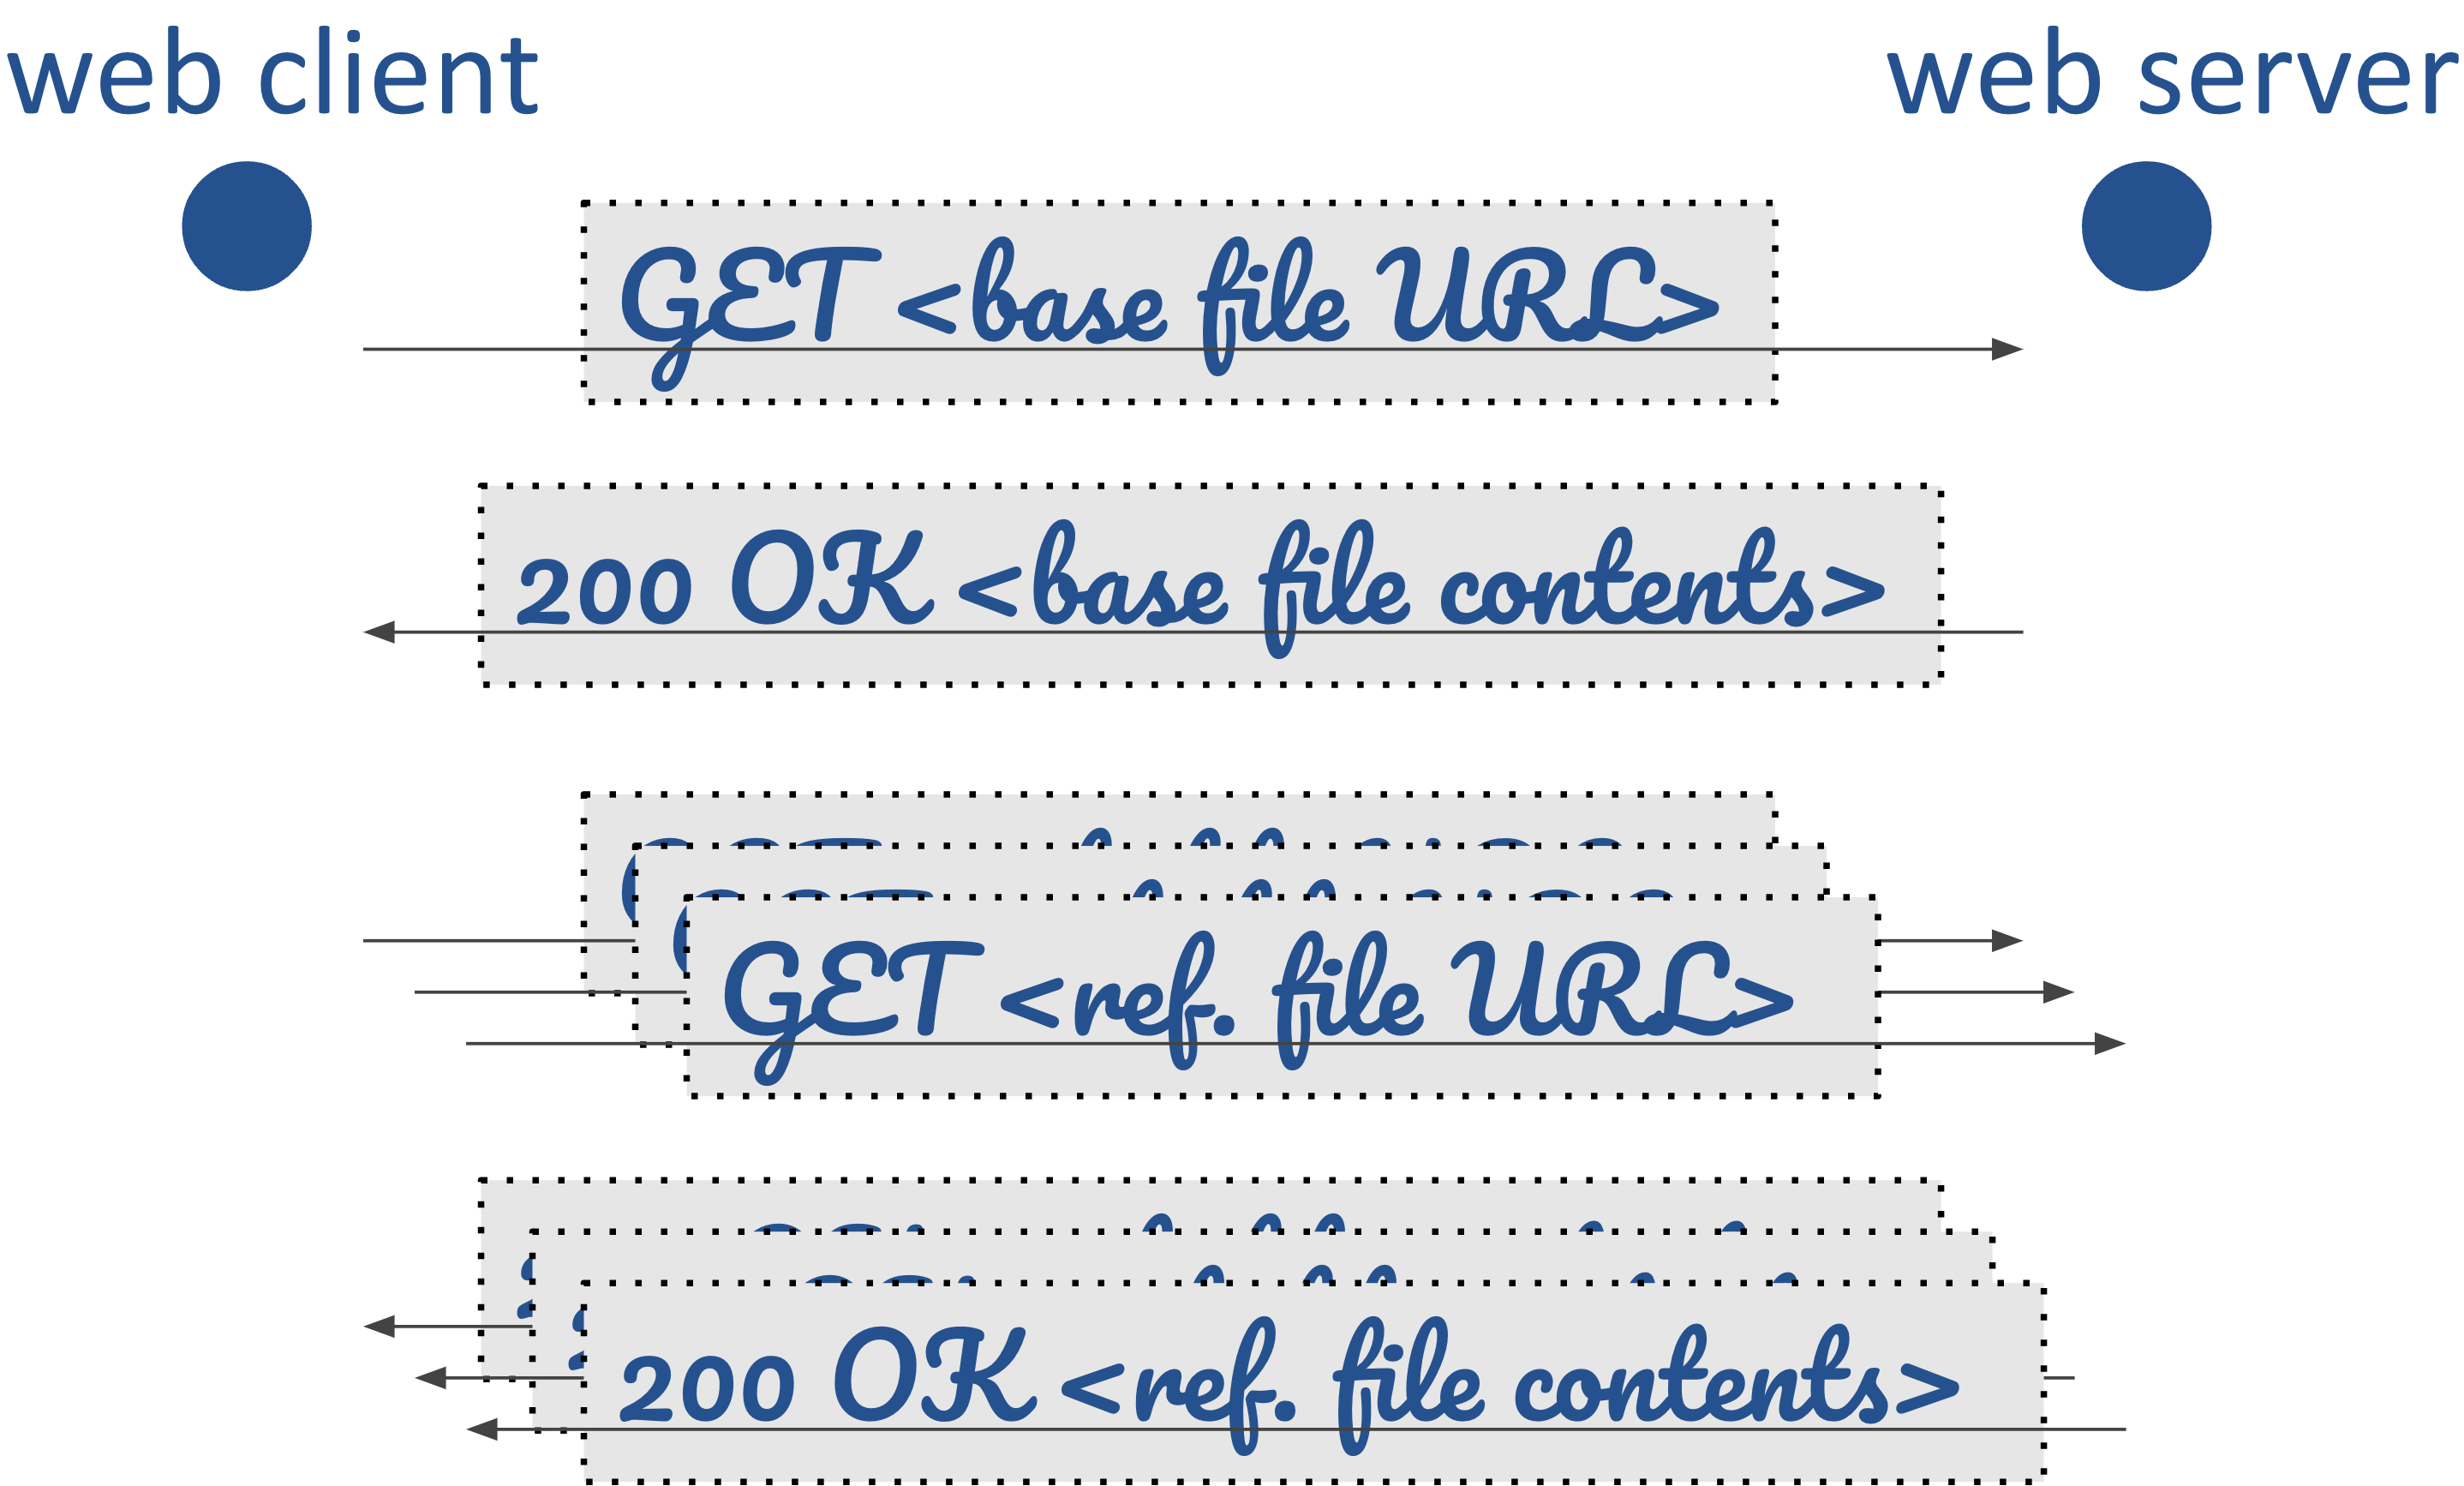
\includegraphics[width=\textwidth]{images/common.png}
\end{center}
\end{minipage}
\hfill
\begin{minipage}[htp]{0.45\textwidth}
\small
\begin{itemize}
    \item A human user types a URL into their web client (e.g., a browser).
    \item The web client sends a \texttt{GET} request for the URL, which identifies the base file of a web page.
    \item The web server responds with a \texttt{200 OK} status, including the content of the requested base file.
    \item The web client parses the base file, discovers all additional URLs (e.g., images, scripts, stylesheets) needed to display the page, and sends a \texttt{GET} request for each one.
\end{itemize}
\end{minipage}

\vspace{10pt}

\noindent
When you visit a web page, your web client sends multiple \texttt{GET} requests to the web server and receives multiple responses to fully render the page.

\subsection{Stateless Protocols}

\begin{itemize}
    \item A server process does \textbf{not} maintain any information (or \textit{state}) about previous interactions with a client.
    \item Here, \textit{state} means data saved from past communication exchanges.
    \item By design, HTTP is a \textbf{stateless} protocol: each request from a client to a server is treated independently.
\end{itemize}
\noindent
Let us contrast \textbf{stateless} versus \textbf{stateful} protocols:

\begin{itemize}
    \item In a \textit{stateful} interaction, the server remembers past conversations and can tailor responses accordingly.
    \item For example, in human conversation (like a classroom lecture), we recall previous topics discussed.
    \item In contrast, some services like a hospital system can be stateless: a new doctor might ask you to explain your medical history again because no information was saved.
\end{itemize}
\noindent
If HTTP is stateless, then how do websites like Facebook or Amazon recognize you when you return, sometimes even before you log in?

\subsection{Example: How Cookies Enable State}
Suppose you open your web client and enter the URL \texttt{news.com/greece.html}.
\begin{center}
    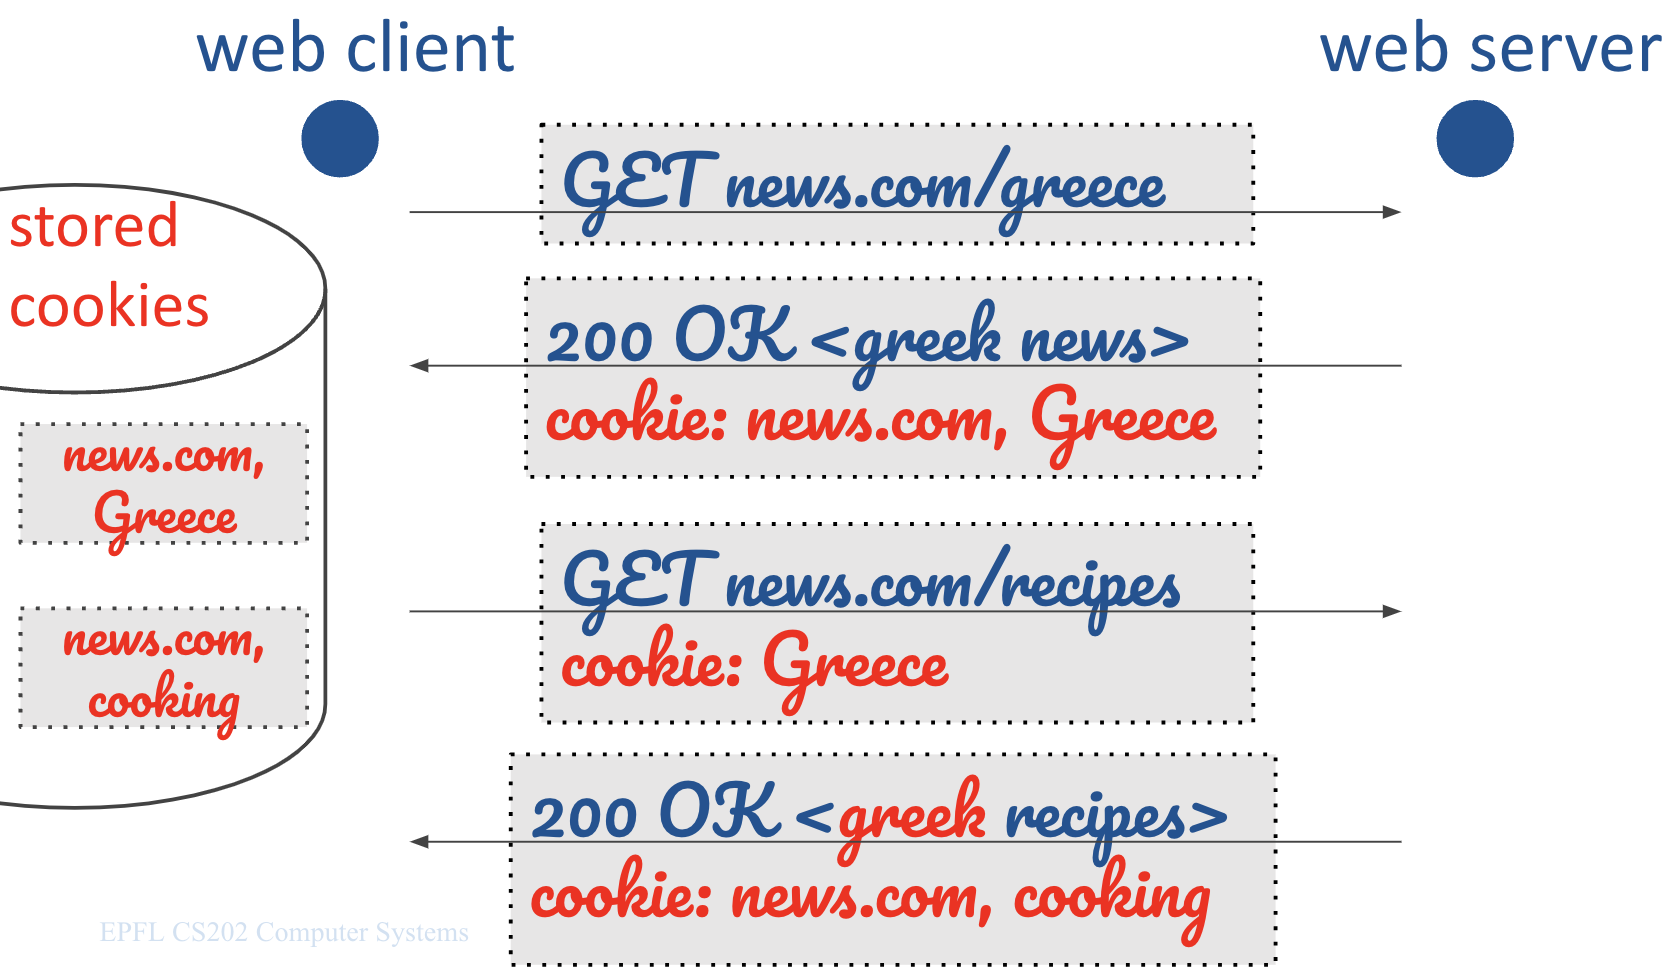
\includegraphics[width=0.6\textwidth]{images/cooking.png}
\end{center}
\begin{quote}
\begin{itemize}
    \item[-] Your web client sends a \texttt{GET} request to \texttt{news.com} for the page \texttt{greece.html}.
    \item[-] The web server responds with the page content and includes a \textbf{cookie} — a small piece of metadata that carries information about you or your preferences (in this case, that you are interested in Greece).
    \item[-] Your web client stores this cookie.
    \item[-] On subsequent requests to \texttt{news.com}, your client sends this cookie back to the server.
    \item[-] The server reads the cookie, learns your interest in Greece, and can customize the response (e.g., show Greek recipes).
    \item[-] The server can update or add new cookies to store additional inferred interests.
\end{itemize}

Over time, the server builds a profile about you based on cookies stored on your client, enabling a personalized experience despite HTTP being stateless.
\end{quote}

\section{Cookies}
Cookies represent \textbf{state created by the web server but stored on the web client}. They serve as a mechanism to link multiple web requests from the same client, enabling session continuity despite HTTP's stateless nature. Through cookies, websites can recognize returning visitors and maintain user preferences across multiple visits.

\subsection{Passing State to the Client}
\begin{itemize}
    \item[-] Instead of storing client-specific information on the server, the server \textbf{passes} that state to the client.
    \item[-] The client stores this state (in cookies) and sends it back on future requests.
    \item[-] This approach reduces server memory and storage requirements.
    \item[-] It also simplifies server design by offloading state management to the client.
\end{itemize}

\paragraph{Professor's Analogy (quoted):} 

When I lived in Greece, clubs charged entrance fees but did not give out tickets. Instead, they stamped a client's forearm. If the client left and returned (e.g., to smoke), showing the stamp proved they had already paid.\\
Here, the club "passed the state to the client" by letting the client carry the proof themselves, rather than maintaining a list or checking IDs repeatedly. This simplified the job and reduced the club's need to keep state information.\\
\noindent
Similarly, cookies pass state information from servers to clients, enabling a stateless HTTP protocol to behave like a stateful system.\\
\textbf{Example of Cross-Site Information Transfer}:\\
\textit{Continuing the previous example:}
\begin{itemize}
    \item \textbf{Initial Visit \& Cookie Association}:
        A web client visits `news.com`. The response from the `news.com` server (or an embedded element therein) causes the client's browser to store a cookie that is associated with a different server, say `cooking.com`.

    \item \textbf{Subsequent Visit to Different Server}:
        When the client later sends its first HTTP request to `cooking.com`, the browser automatically includes this specific cookie with the request.

    \item \textbf{Information Gained by Third Party}:
        As a result, the `cooking.com` server receives this cookie. It can then learn information about the client (e.g., an inferred interest in "Greece," perhaps based on the context from `news.com` or the cookie's content itself), even though this is the client's very first direct communication with `cooking.com`.
\end{itemize}

\subsection{Third-Party Cookies}
A \textbf{third-party cookie} is a cookie set by a web server for a domain different from the one the user is currently visiting. This allows information about a user's browsing activity to be shared across different websites.

\begin{itemize}
    \item \textbf{Definition}: A cookie created by one web server (e.g., an ad network) to be used when the client visits web pages hosted by other, different web servers.
    \item \textbf{Mechanism}:
    \begin{enumerate}
        \item A user visits `news.com`. The `news.com` server's response might include instructions for the browser to fetch content from `ads.com` (e.g., an image or script).
        \item When the browser requests content from `ads.com`, `ads.com` can set a cookie in the user's browser. This is a third-party cookie from the perspective of `news.com`.
        \item Later, if the user visits `cooking.com`, and `cooking.com` also embeds content from `ads.com`, the browser will send the cookie previously set by `ads.com` along with the request to `ads.com`.
    \end{enumerate}
    \item \textbf{Implication}: The third-party server (`ads.com`) can track the user's visits across multiple sites (`news.com`, `cooking.com`), building a profile of their interests even if the user has never directly visited the third-party's website.
\end{itemize}

\subsection{Cookie-less Tracking}
\textbf{Cookie-less tracking} refers to techniques used by web servers to collect information about web clients and their activities without relying on traditional HTTP cookies.

\begin{itemize}
    \item \textbf{Methods}: These can include browser fingerprinting (collecting unique browser configurations), IP address tracking, ETags, or other header information.
    \item \textbf{Privacy Considerations}:
    \begin{itemize}
        \item A common misconception is that cookie-less tracking is inherently more privacy-preserving simply because it avoids cookies.
        \item \textbf{This is not necessarily true.} Cookies are just one mechanism for user profiling. The critical factor for privacy is the \textit{nature and extent of the information collected and how it is used}, not the specific mechanism (cookies or otherwise).
        \item Cookie-less \textit{tracking} is still \textit{tracking}. Its impact on privacy depends on what data is gathered and for what purpose.
    \end{itemize}
\end{itemize}
\newpage

\section{Web Caching}
Web caching is a core technique for improving the performance of web applications by storing copies of frequently accessed resources closer to the user.

\subsection{Introduction to Web Caching}
\begin{itemize}
    \item A \textbf{web cache} (or \textbf{proxy web server}) is an intermediary server that stores (caches) copies of web content (e.g., HTML pages, images, files) served by origin web servers.
    \item It acts as a server to nearby web clients and as a client to the origin web servers.
    \item \textbf{Primary Goals}:
    \begin{itemize}
        \item \textbf{Reduce Delay}: Clients experience faster load times as content is retrieved from a geographically closer cache rather than a distant origin server.
        \item \textbf{Reduce Load on Origin Server}: Fewer requests reach the origin server, decreasing its workload and bandwidth consumption.
    \end{itemize}
\end{itemize}
\begin{center}
    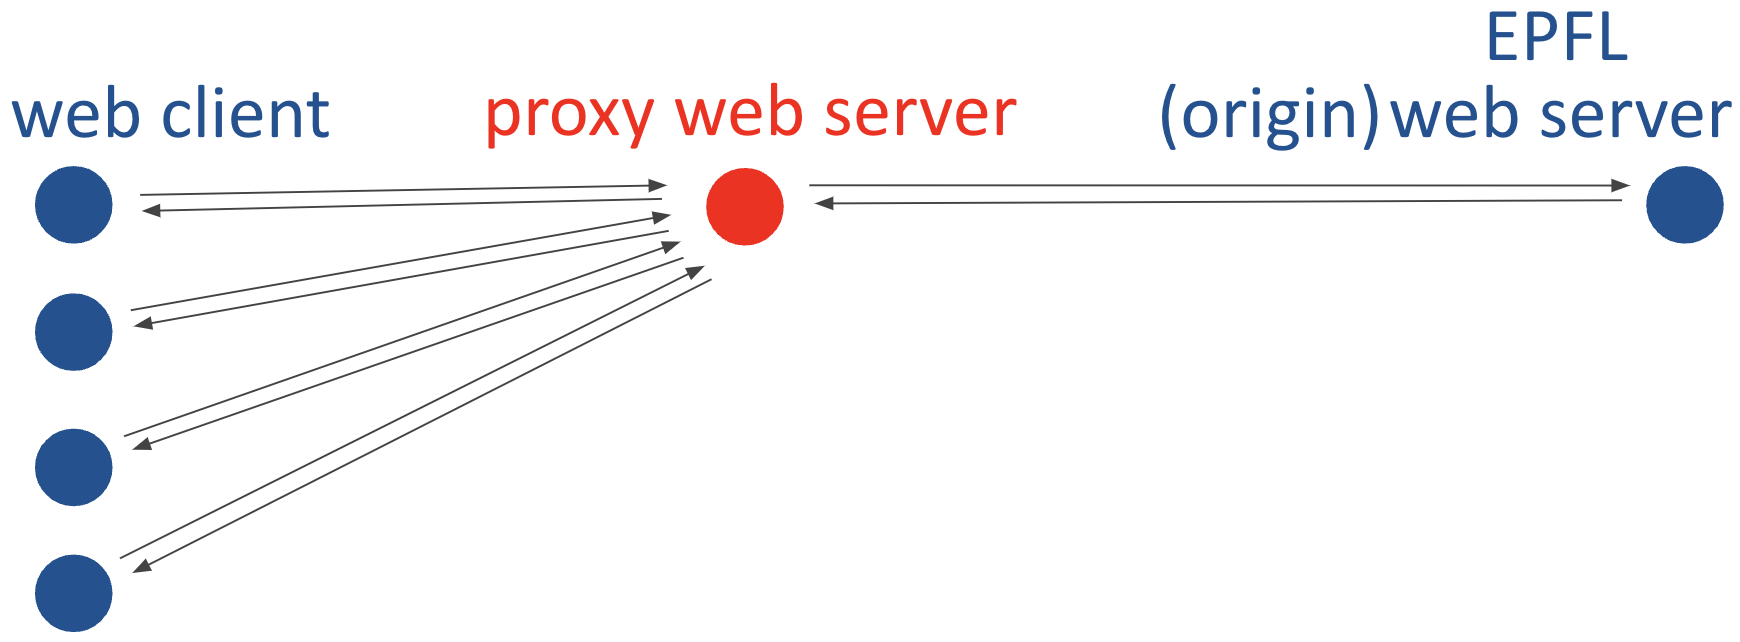
\includegraphics[width=0.6\textwidth]{images/caching.png} % Ensure this image is in a subdirectory 'images' or adjust path
\end{center}

\subsection{Web Caching Mechanism: An Example}
Consider a web client accessing a resource (e.g., `www.example.com/resource`) from a distant origin server. A local proxy web server can be used:
\begin{enumerate}
    \item \textbf{First Client Request (Cache Miss)}:
    \begin{itemize}
        \item Client 1 sends a GET request for the URL to the nearby proxy server.
        \item The proxy checks its local cache. If the resource is not found (a \textbf{cache miss}), the proxy forwards the GET request to the origin server.
        \item The origin server responds to the proxy with the resource.
        \item The proxy stores a copy of the resource in its cache and forwards the resource to Client 1.
        \item Client 1 experiences a delay, potentially slightly longer due to the intermediary step.
    \end{itemize}
    \item \textbf{Subsequent Client Requests (Cache Hit)}:
    \begin{itemize}
        \item Client 2 (or Client 1 again) requests the same URL from the proxy server.
        \item The proxy checks its cache and finds a fresh copy of the resource (a \textbf{cache hit}).
        \item The proxy immediately sends the cached resource to Client 2, without contacting the origin server.
        \item Client 2 experiences significantly reduced delay.
    \end{itemize}
\end{enumerate}

\subsection{Challenge: Ensuring Data Freshness}
A critical challenge in web caching is ensuring that the cached data is not \textbf{stale} (i.e., an outdated version of the resource). Clients should receive the most current version.

\subsubsection{Cache Validation Mechanisms}
To address stale data, caches use validation mechanisms:
\begin{itemize}
    \item \textbf{Expiration Time / Max Caching Age}:
    \begin{itemize}
        \item Origin servers can include HTTP headers in their responses to specify how long a resource can be considered fresh.
            \item `Expires`: Provides a specific date/time after which the resource is stale.
            \item `Cache-Control: max-age=<seconds>`: Specifies the maximum time in seconds that the resource can be cached without revalidation.
        \item Once this period elapses, the cache considers its copy stale.
    \end{itemize}
    \item \textbf{Conditional GET Requests}:
    \begin{itemize}
        \item When a cached resource is stale (or if the cache wants to verify freshness), it can send a \textbf{conditional GET request} to the origin server.
        \item This request asks the server to send the resource \textit{only if it has been modified} since the version stored in the cache.
        \item The `If-Modified-Since` HTTP request header is used, containing the `Last-Modified` timestamp of the cached version.
        \begin{center}
        \texttt{GET /resource.html HTTP/1.1 \\
        Host: www.example.com \\
        If-Modified-Since: Wed, 21 Oct 2023 07:28:00 GMT}
        \end{center}
        \item \textbf{Server Response}:
            \begin{itemize}
                \item If the resource \textit{has not been modified} since the specified date, the origin server responds with `HTTP/1.1 304 Not Modified`. This response has no body, saving bandwidth. The cache can then serve its stored copy.
                \item If the resource \textit{has been modified}, the origin server responds with `HTTP/1.1 200 OK` and the new version of the resource, which the cache then stores and forwards to the client.
            \end{itemize}
    \end{itemize}
\end{itemize}
\begin{center}
    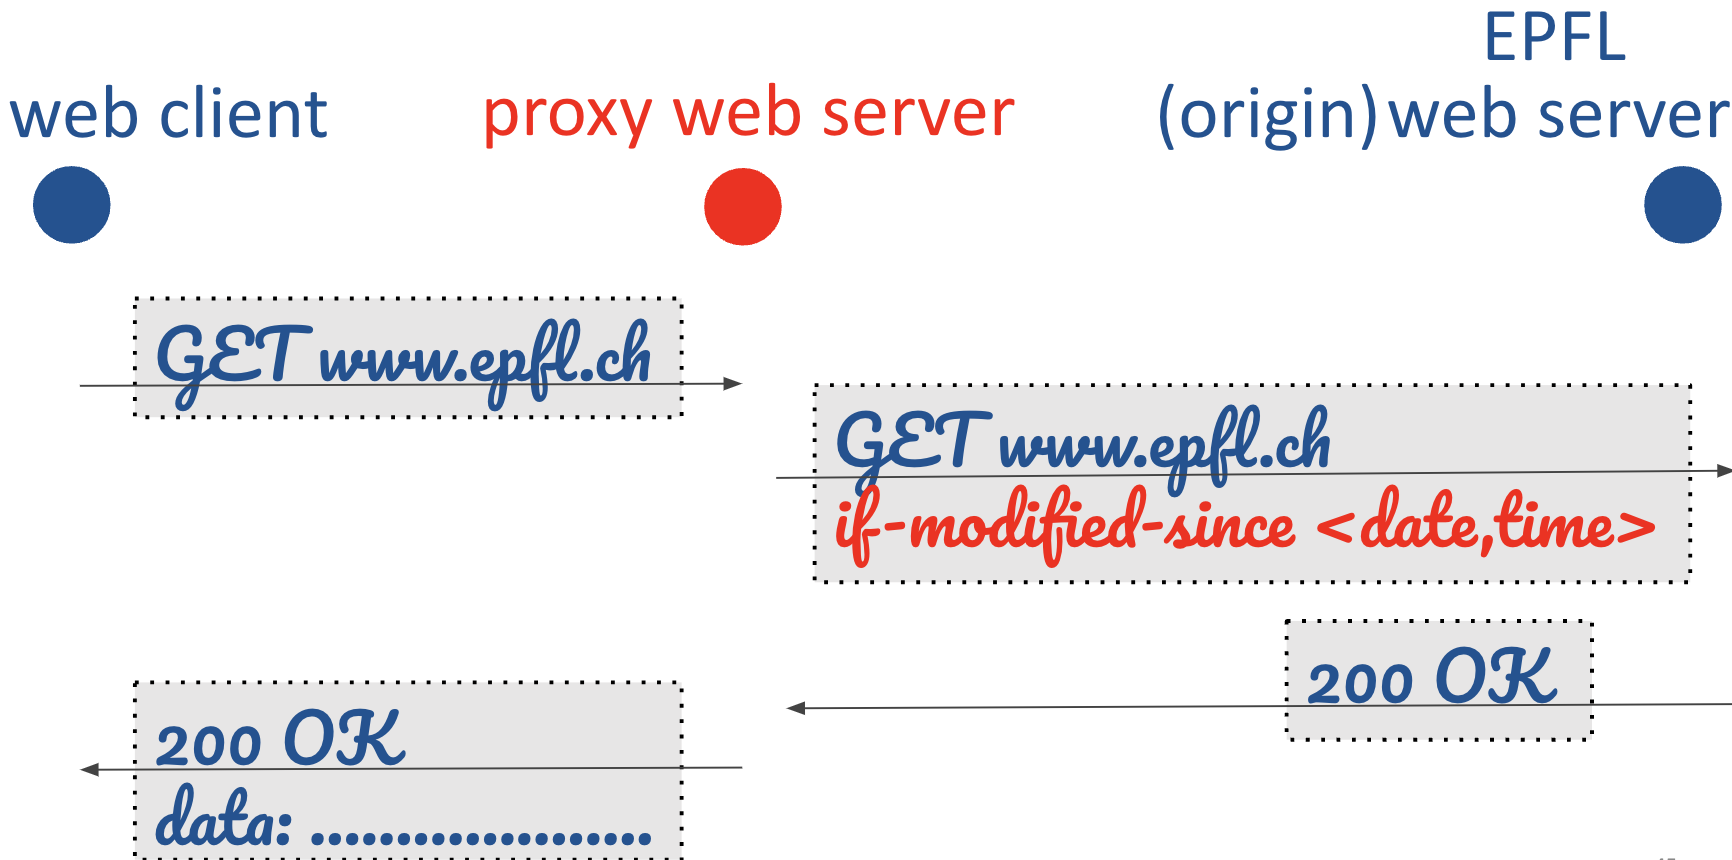
\includegraphics[width=0.6\textwidth]{images/cache-age.png} % Ensure this image is in a subdirectory 'images' or adjust path
\end{center}
\textit{Note: Web clients (browsers) also maintain their own local caches and employ similar mechanisms (expiration policies, conditional GETs) for resources they fetch.}

\subsection{Impact of Conditional GET on Performance}
Does a conditional GET request significantly reduce delay?
\begin{itemize}
    \item \textbf{Not always significantly for delay}: A conditional GET still requires a round-trip to the origin server to check for modifications. If the object is small, the time saved by not re-downloading it (in case of a `304 Not Modified`) might be marginal compared to the round-trip time itself.
    \item \textbf{Significant for bandwidth and large objects}: If the requested object is large, receiving a `304 Not Modified` response avoids re-transmitting the entire object, leading to substantial savings in bandwidth and a noticeable reduction in delay compared to a full download.
\end{itemize}

\subsection{General Principles of Caching}
\begin{itemize}
    \item Caching is a \textbf{universal technique} for improving performance in systems where data is accessed repeatedly.
    \item \textbf{Core Idea}: When one entity incurs the cost to fetch data, cache it locally (or closer to other potential consumers) so that subsequent requests for the same data can be served faster and with less resource consumption on the origin.
    \item \textbf{Primary Challenge}: Ensuring \textbf{data freshness} or \textbf{cache coherency}—that the cached data accurately reflects the current state of the origin data.
    \item \textbf{Common Solutions}:
    \begin{itemize}
        \item Assigning an \textbf{expiration date} or \textbf{max caching age} to data.
        \item Performing \textbf{dynamic checks} (e.g., conditional GETs) with the origin source to validate freshness. The utility of dynamic checks can depend on factors like data size and communication overhead.
    \end{itemize}
\end{itemize}


\end{document}